\chapter{Writing Your First Prompt: From Text to Video}
\label{ch:first-Prompt}

\begin{chapterabstract}
This chapter establishes the foundational principles of Prompt engineering for Sora 2, teaching readers how to transform textual descriptions into compelling visual narratives. We introduce the concept of Prompts as ``narrative visual construction grammar''—a system that merges literary rhythm with photographic logic. The chapter presents a structured four-step methodology covering setting, action, camera work, and emotion, providing systematic frameworks for constructing effective Prompts. We explore the three layers of Prompt meaning: the literal layer (visible elements), the cinematic layer (camera techniques and composition), and the emotional layer (atmosphere and psychological undertones). Through annotated examples and comparative analysis, readers learn to write Prompts that communicate not just content but directorial intent. The chapter addresses common beginner mistakes, including over-specification, conflicting instructions, and emotional ambiguity. Practical exercises guide readers through progressive skill development, from simple scene descriptions to complex multi-element compositions. By mastering these fundamentals, readers establish the technical vocabulary and conceptual framework necessary for advanced Prompt engineering explored in later chapters.
\end{chapterabstract}

You've opened Sora 2, created your first project, and the cursor blinks in the Prompt box. This is the starting point of creation---a line of text is about to ignite the birth of a visual experience. For beginners, this moment feels like entering an unknown wilderness and stepping behind the scenes of cinema. The blank Prompt box is the stage, and your words are the collective instructions for lighting, camera, and actors.

In this chapter, we will not only discuss ``how to write,'' but also understand ``why to write this way.'' Sora 2 Prompts are not just language describing objects, but a textual extension of directorial thinking---connecting imagination with algorithms, poetry with logic. You will learn how to turn a sentence into a film, making the system not just ``understand'' your words, but ``feel'' your intention.

\section{The True Meaning of Prompts: From Language to Shots}
\index{Prompts!definition}
\index{cinematic language}

In the world of Sora 2, text is cinematic language. A Prompt is not a command, but a \textbf{narrative visual construction grammar}\index{visual grammar}. It merges the rhythm of literature with the logic of photography: requiring both content accuracy and atmospheric extensibility. Good Prompts are visual seeds that can grow light, shadow, and emotion within algorithms.

We can break down the meaning of Prompts into three layers:

\begin{enumerate}
\item \textbf{Literal Layer}: Elements appearing in the frame---characters, objects, scenes, props, weather, etc.
\item \textbf{Cinematic Layer}\index{cinematic layer}: Camera angle, movement method, shot size, focal length, rhythm, and composition
\item \textbf{Emotional Layer}\index{emotional layer}: Overall tone, psychological undercurrent, story atmosphere, audience expectations
\end{enumerate}

The relationship between these three is like the three major elements of film---script, photography, and music. When they are harmoniously aligned, Sora 2 can generate shots with a sense of life.

For example:

\begin{Prompt}
``A young woman rides a bicycle through narrow streets at dusk, the camera gliding beside her, wind tousling her hair, her laughter echoing in the sunset.''
\end{Prompt}

\begin{figure}[H]
\centering
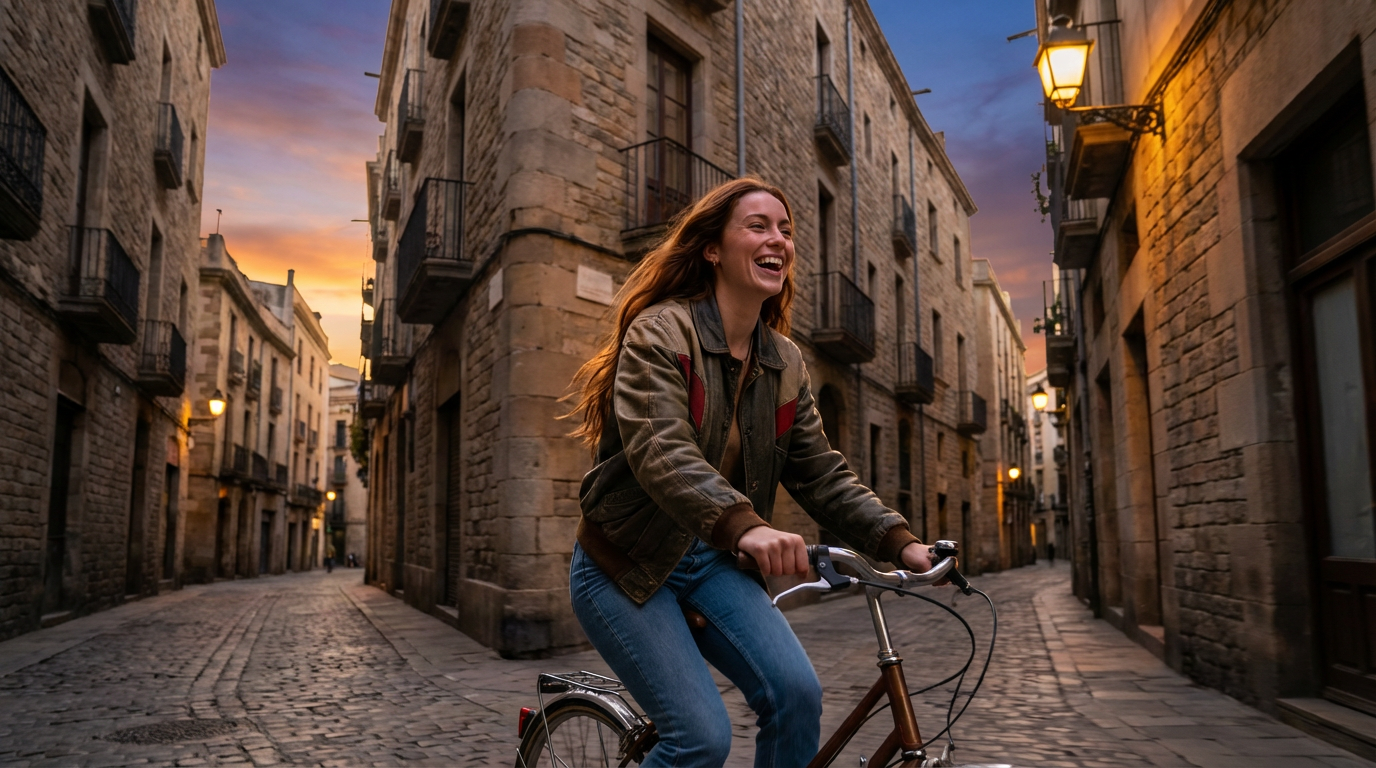
\includegraphics[height=\figheight]{Fig3-1.png}
\caption{Dynamic composition showing movement and emotional connection \\ \authorcreated}
\label{fig:ch03-bicycle}
\end{figure}

This sentence contains signals from all three layers: \textbf{environment} (dusk, narrow streets), \textbf{movement} (cycling, gliding), \textbf{emotion} (freedom, warmth, wind sensation). Sora 2 will automatically fill in light direction, camera distance, color temperature, and rhythm.

Conversely, if you only input ``a woman riding a bicycle,'' the algorithm cannot determine whether she's exercising in the morning, escaping, traveling, or dreaming. The loss of cinematic quality often isn't due to AI capability, but due to the lack of layered Prompts.

\section{Basic Structure of Prompts: The Four-Step Method}
\index{Prompt structure}
\index{four-step method}

A complete cinematic Prompt should contain at least the following four elements:

\begin{enumerate}
\item \textbf{Setting}---Where are we? When? What lighting?
\item \textbf{Action}---Who is doing what? Fast or slow rhythm?
\item \textbf{Camera}---From which angle? Handheld, tracking, or aerial?
\item \textbf{Tone}---What should the audience feel? Gentle? Tense? Lonely?
\end{enumerate}

You can naturally integrate these elements into sentences without being constrained by order. For example:

\begin{Prompt}
``At dawn on snowy ground, a fox slowly walks past, the camera follows at low angle, its footprints extending a lonely rhythm in the morning light.''
\end{Prompt}

\begin{figure}[H]
\centering
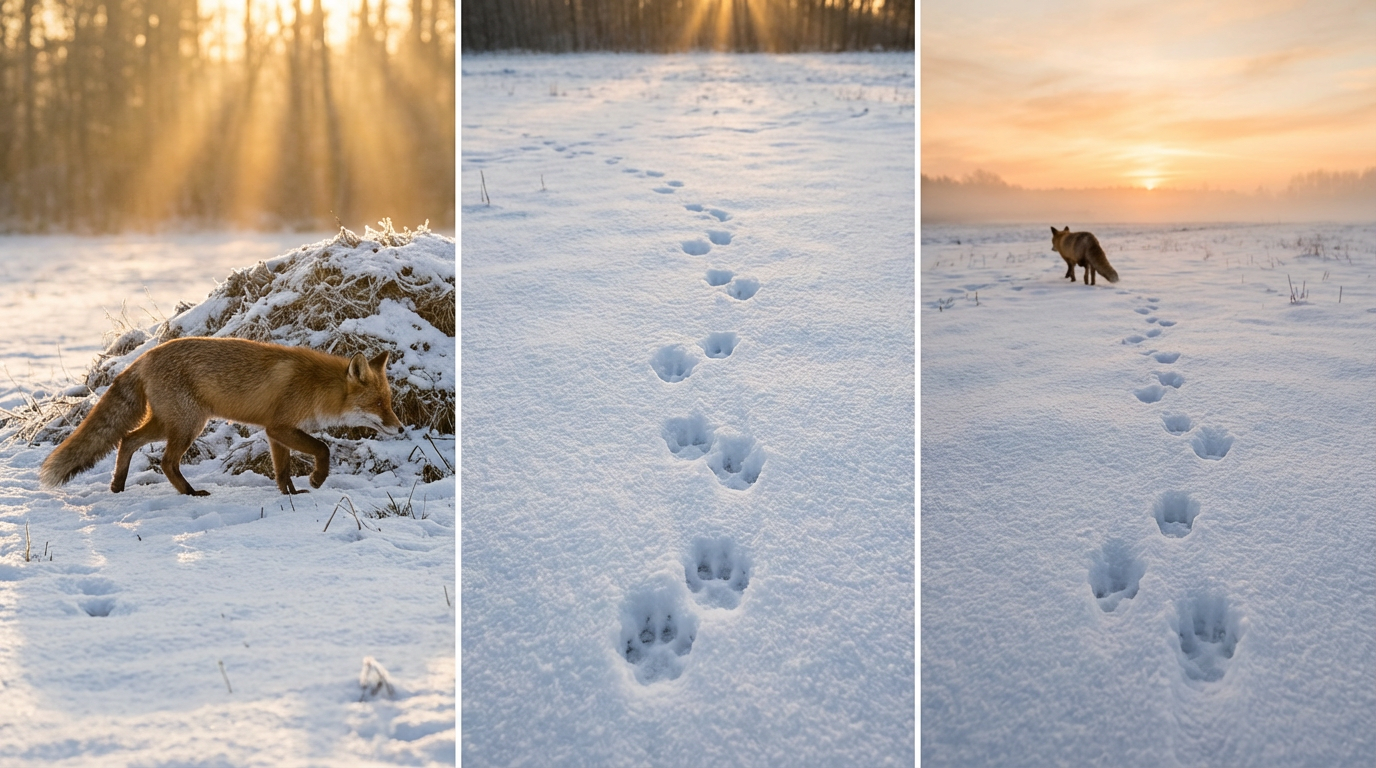
\includegraphics[height=\figheight]{Fig3-2.png}
\caption{Low-angle tracking shot creating atmospheric storytelling \\ \authorcreated}
\label{fig:ch03-fox}
\end{figure}

In this text, Sora 2 will not only generate visuals but also capture rhythm: snow brightness, pace speed, camera low-position movement, cold and quiet atmosphere.

Prompts are like a river, each clause a change in flow rate. Mastering structure means mastering rhythm.

\section{Sentence Patterns and Rhythm: Editing Film with Text}
\index{sentence rhythm}
\index{visual tempo}

Film rhythm is often hidden in language structure. Sora 2 judges shot transitions or continuity based on commas, periods, and subordinate clauses.

\begin{itemize}
\item \textbf{Short sentences}: Quick cuts, creating tension and impact
\item \textbf{Long sentences}: Smooth continuous shots, creating immersion and lyricism
\end{itemize}

\textbf{Example 1 (Fast rhythm):}

\begin{Prompt}
``Rain. Sirens. Footsteps. Man turns back. Lights flicker.''
\end{Prompt}

\begin{figure}[H]
\centering
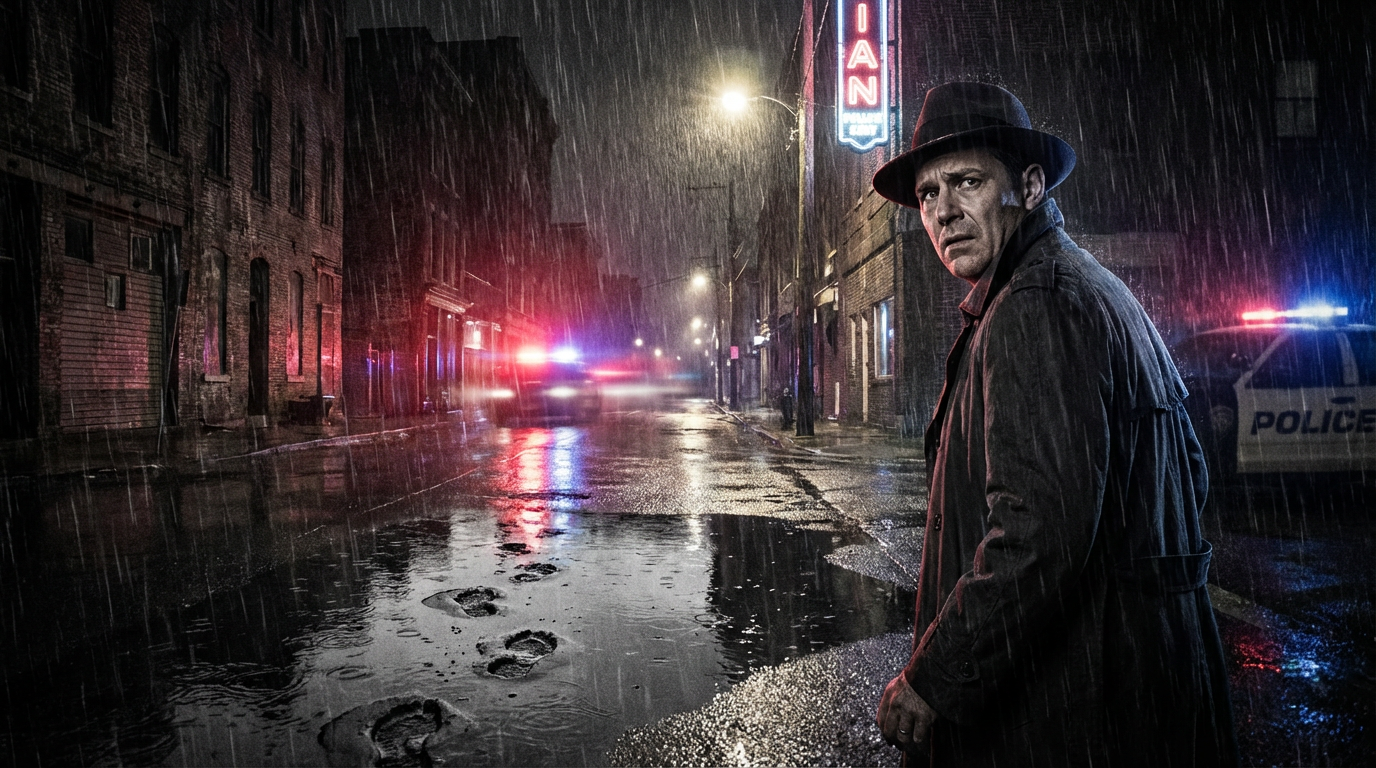
\includegraphics[height=\figheight]{Fig3-3.png}
\caption{Staccato visual rhythm creating urgency \\ \authorcreated}
\label{fig:ch03-rain-sirens}
\end{figure}

\textbf{Example 2 (Slow rhythm):}

\begin{Prompt}
``Sunset filters through dusty windows, light dancing on book pages, air stands still.''
\end{Prompt}

\begin{figure}[H]
\centering

\includegraphics[height=\figheight]{Fig3-4.png}
\caption{Long take with soft focus and warm light creating nostalgic mood \\ \authorcreated}
\label{fig:ch03-sunset-window}
\end{figure}

In creation, you can use \textbf{punctuation to control time}. Commas represent ``camera breathing,'' periods represent ``cut to new shot.'' When sentence rhythm aligns with visual rhythm, AI-generated segments exhibit natural cadence.

\section{Light and Color: Emotional Codes of Visual Narrative}
\index{lighting!emotional language}
\index{color theory}

In Sora 2's understanding system, light is the language of emotion. When you use ``warm'' and ``cold,'' you're adjusting color temperature; when you write ``moonlight,'' ``neon,'' ``firelight,'' you're defining light sources. AI will choose contrast, saturation, shadow layers, and reflection relationships accordingly.

\textbf{Example comparison:}

\begin{Prompt}
``A boy writes a letter under warm lamplight, soft jazz floating through the room.''
\end{Prompt}

\begin{figure}[H]
\centering

\includegraphics[height=\figheight]{Fig3-5.png}
\caption{Warm lighting establishing intimate atmosphere \\ \authorcreated}
\label{fig:ch03-warm-lamp}
\end{figure}

$\rightarrow$ Temperature, music, and rhythm unified, creating cozy ambiance.

\begin{Prompt}
``A boy reviews under harsh fluorescent light, the clock's second hand crisply striking the air.''
\end{Prompt}

\begin{figure}[H]
\centering
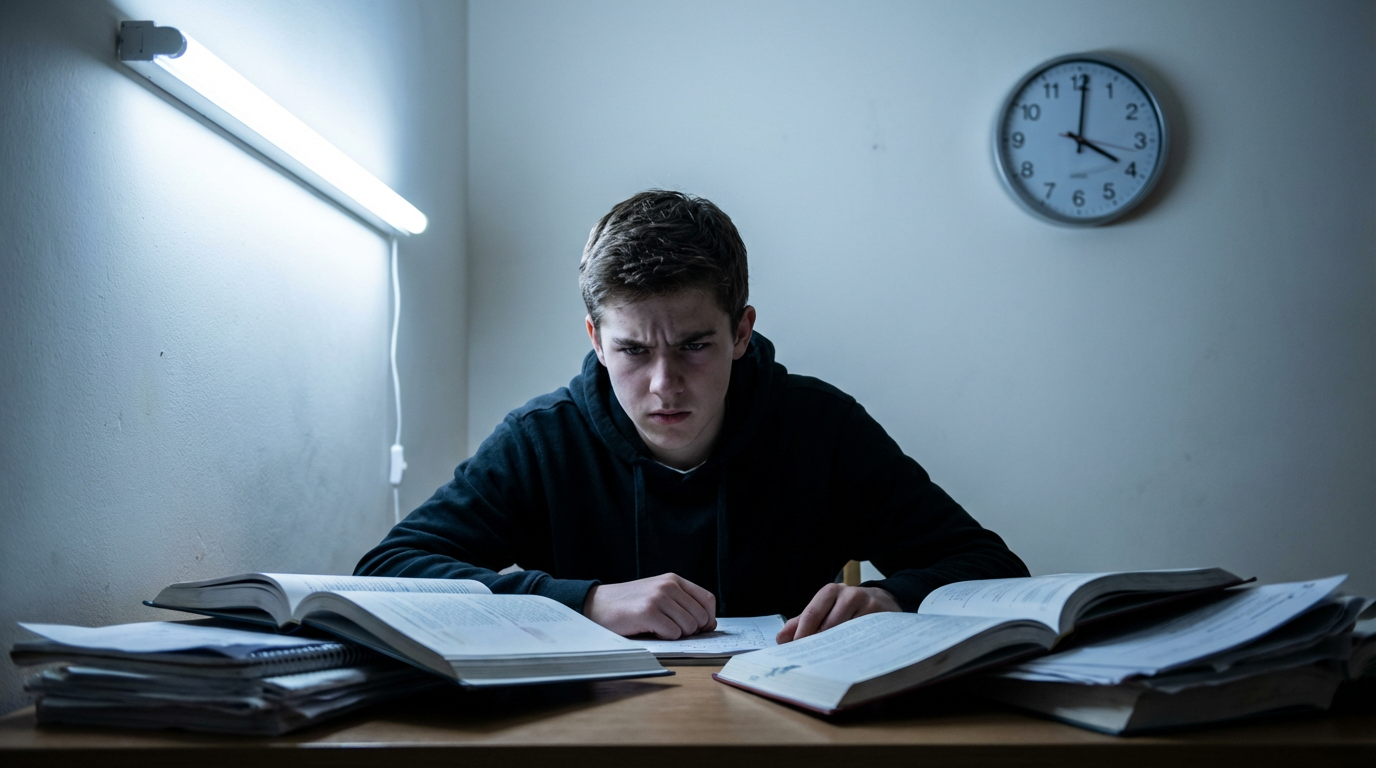
\includegraphics[height=\figheight]{Fig3-6.png}
\caption{Harsh lighting creating isolation and pressure \\ \authorcreated}
\label{fig:ch03-harsh-light}
\end{figure}

$\rightarrow$ Same scene, but becomes a symbol of loneliness and oppression.

You can use light to control temporal feeling. For example: ``orange morning light'' suggests hope at dawn, ``blue-gray light'' implies night's oppression, ``silver moonlight'' evokes dreams and distance. AI is extremely sensitive to these adjectives; a single word can rewrite the entire visual rhythm.

\section{Cinematographic Language: Giving Images Directorial Presence}
\index{cinematographic techniques}
\index{camera movements}

Sora 2 understands numerous photographic terms that you can directly invoke. For example:

\begin{table}[H]
\centering
\caption{Camera Techniques and Their Effects \\ \authorillustration}
\label{tab:camera-techniques}
\begin{tabular}{|l|p{5cm}|p{4cm}|}
\hline
\textbf{Type} & \textbf{Keywords} & \textbf{Effect} \\
\hline
Static shot & Tripod, fixed camera, eye-level & Stable, solemn \\
Tracking shot & Following, pan, dolly & Dynamic, immersive \\
Aerial shot & Bird's-eye view, drone perspective & Grand, detached \\
Close-up & Macro, focus, eyes & Strong emotional tension \\
Handheld & Shaky, immediacy, documentary feel & Authentic, chaotic \\
Push/Pull & Slow zoom, push-pull & Oppressive, transitional, dramatic \\
\hline
\end{tabular}
\end{table}

For example:

\begin{Prompt}
``Handheld close-up, a firefighter's face flickering in firelight, sweat and ash intertwined.''
\end{Prompt}

\begin{figure}[H]
\centering
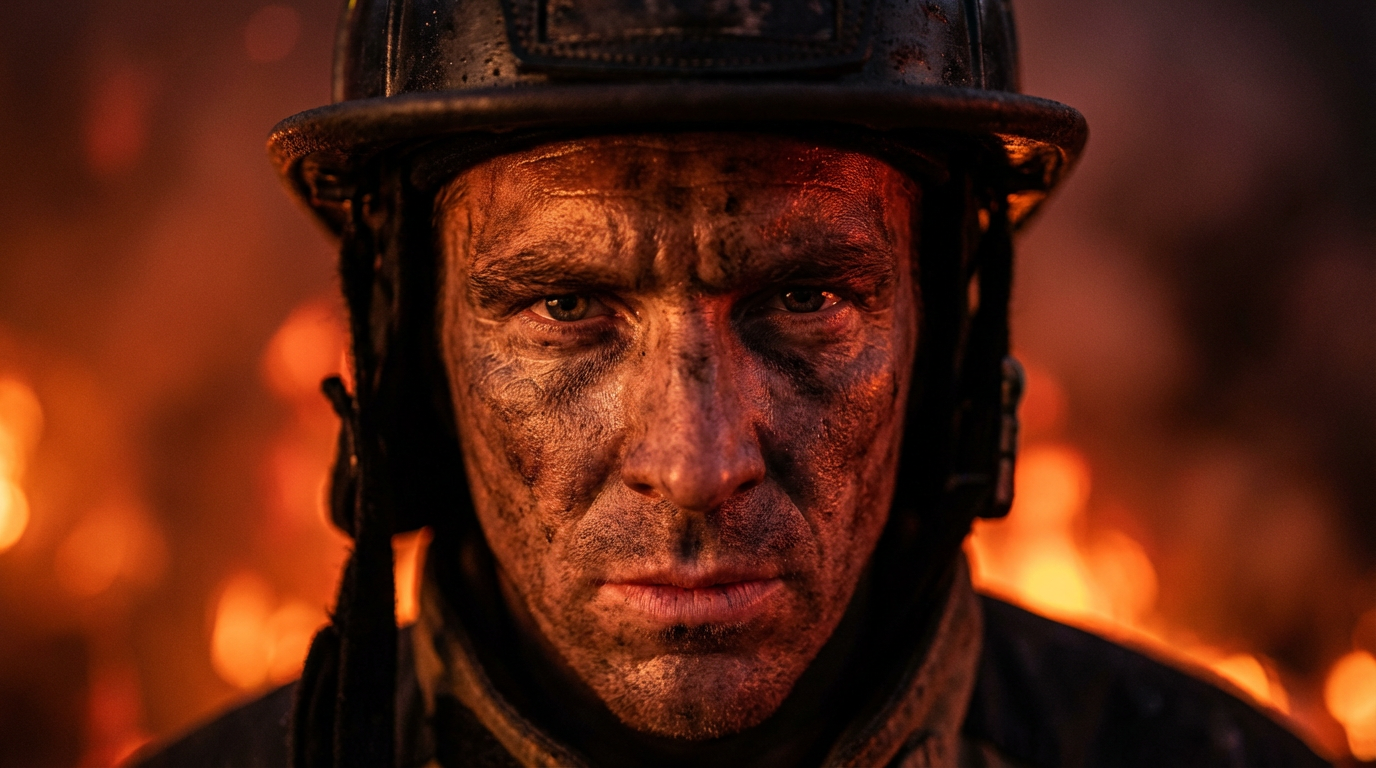
\includegraphics[height=\figheight]{Fig3-7.png}
\caption{Handheld close-up creating immediate emotional intensity \\ \authorcreated}
\label{fig:ch03-firefighter}
\end{figure}

The system will automatically understand: high emotion, close distance, handheld movement, orange-red dominant color.

If changed to:

\begin{Prompt}
``Aerial shot, the city burns into a red map, night torn open.''
\end{Prompt}

\begin{figure}[H]
\centering
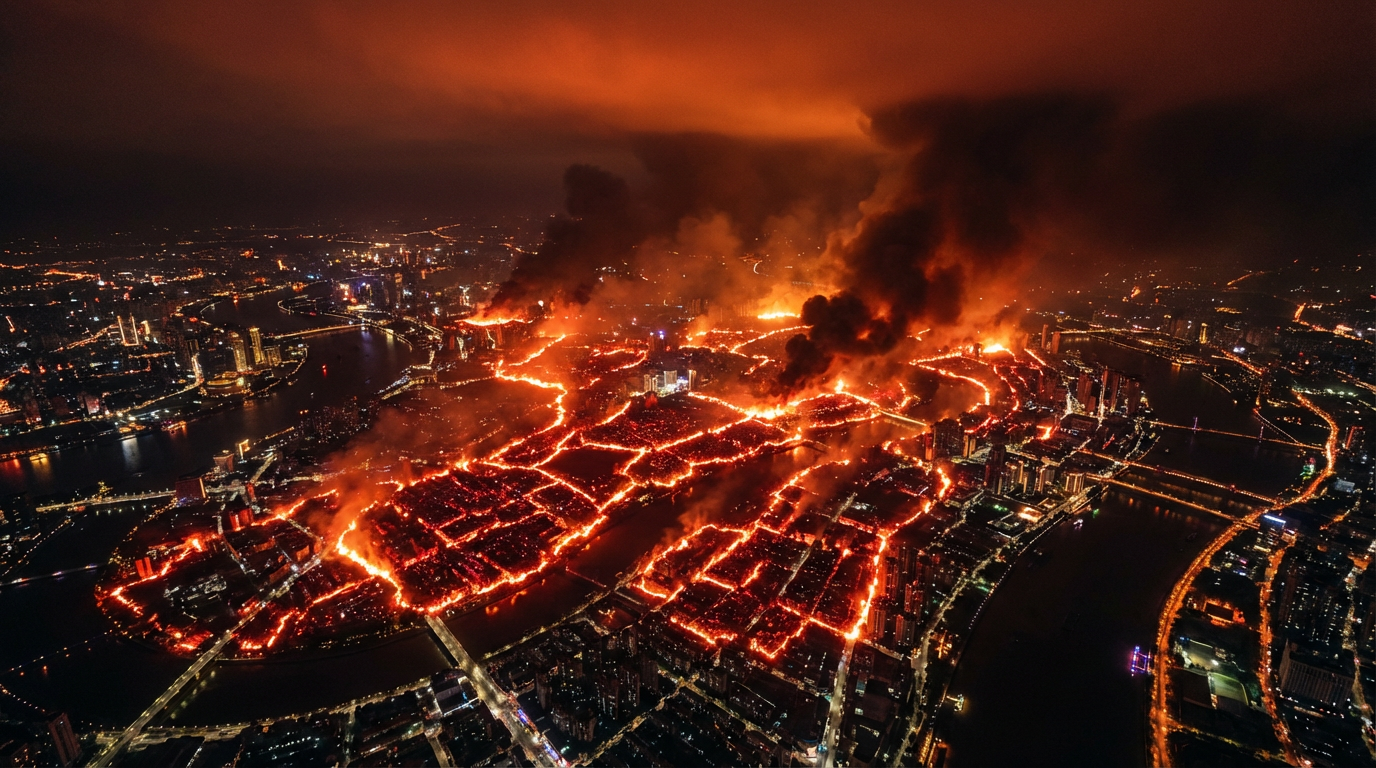
\includegraphics[height=\figheight]{Fig3-8.png}
\caption{Epic aerial perspective transforming narrative scale \\ \authorcreated}
\label{fig:ch03-aerial-city}
\end{figure}

That becomes epic macro-narrative. Different cinematographic language makes the same subject present completely different emotional levels.

\section{Writing Emotion: Making Images Breathe}
\index{emotional writing}
\index{empathy in AI}

AI's core is not generation, but \textbf{empathy}. The emotional words you provide are key clues for it to understand rhythm.

For example:

\begin{Prompt}
``She pushes open the dust-covered door, light pouring in from the gap, as if time trembles.''
\end{Prompt}

\begin{figure}[H]
\centering

\includegraphics[height=\figheight]{Fig3-9.png}
\caption{Metaphorical language creating temporal atmosphere \\ \authorcreated}
\label{fig:ch03-door-light}
\end{figure}

Here, ``as if time trembles'' makes the system understand to slow down, soft focus, low saturation. Emotional words affect not only visuals but also sound design, color tone, and action speed.

Imagine writing ``the emotion of wind''---not just writing wind, but writing ``the touch of wind.'' Sora 2 can read the psychological implications behind ``lonely wind,'' ``scorching wind,'' ``salt-laden wind,'' thereby changing the entire scene's tone.

\section{Iteration and Direction: Balancing Refinement and Rhythm}
\index{iterative refinement}
\index{directorial control}

Excellent Prompts are not achieved in one go but obtained through repeated experimentation. You need to, like a director, continuously adjust rhythm and tone.

The first generation might be too bright, the second too dark, the third with scattered composition. Adjust one variable each time: lighting, camera movement, tonal adjectives, emotional intensity. Observe changes---this is the process of training ``visual intuition.''

\begin{Prompt}
First draft: ``A woman stands on a rainy night street under neon lights, camera slowly rotates.''

Second draft: ``A woman stands in a flickering neon-lit rain alley, rainwater dripping from her fingertips, blue-purple lights reflecting a lonely silhouette.''
\end{Prompt}

\begin{figure}[H]
\centering
\begin{minipage}{0.48\textwidth}
\centering
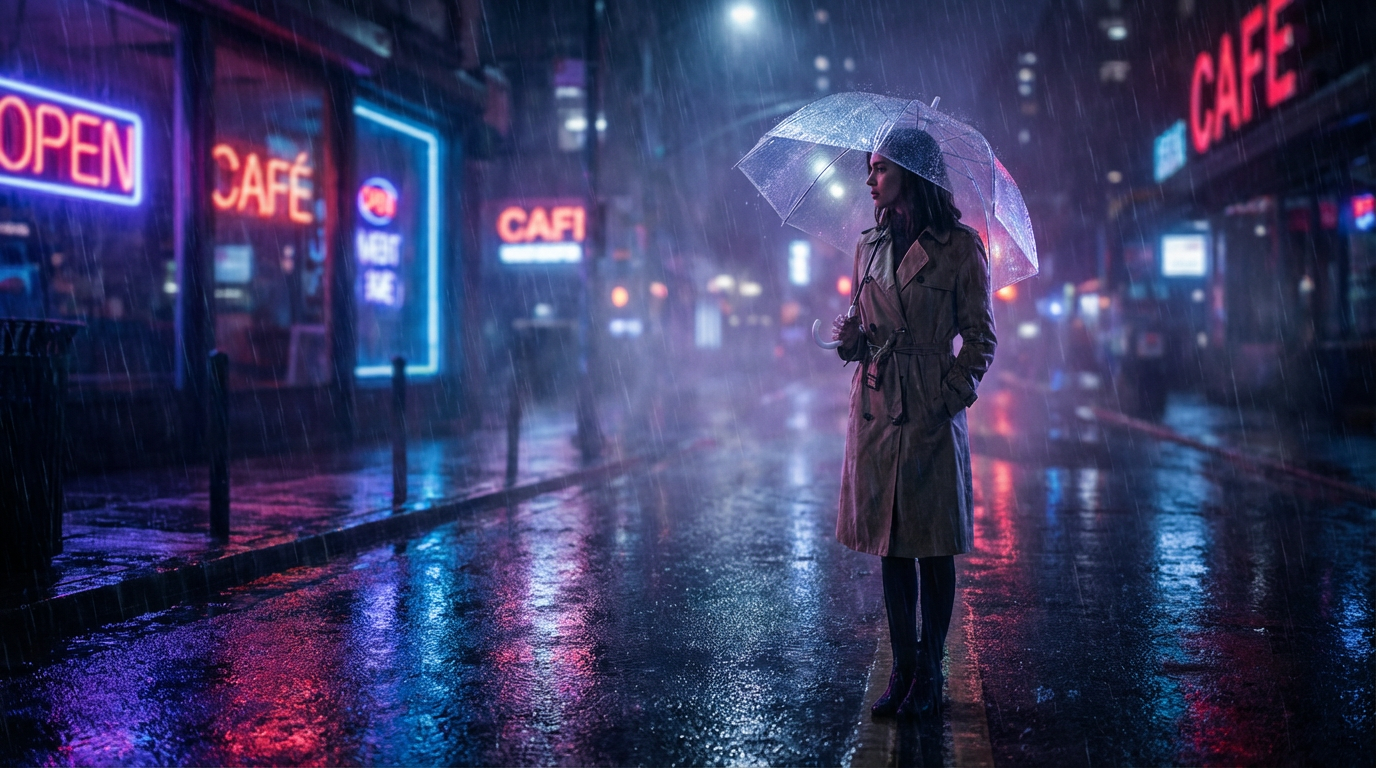
\includegraphics[width=\textwidth]{Fig3-10-1.png}
\subcaption{First draft: Basic scene description}
\label{fig:ch03-neon-rain-v1}
\end{minipage}
\hfill
\begin{minipage}{0.48\textwidth}
\centering
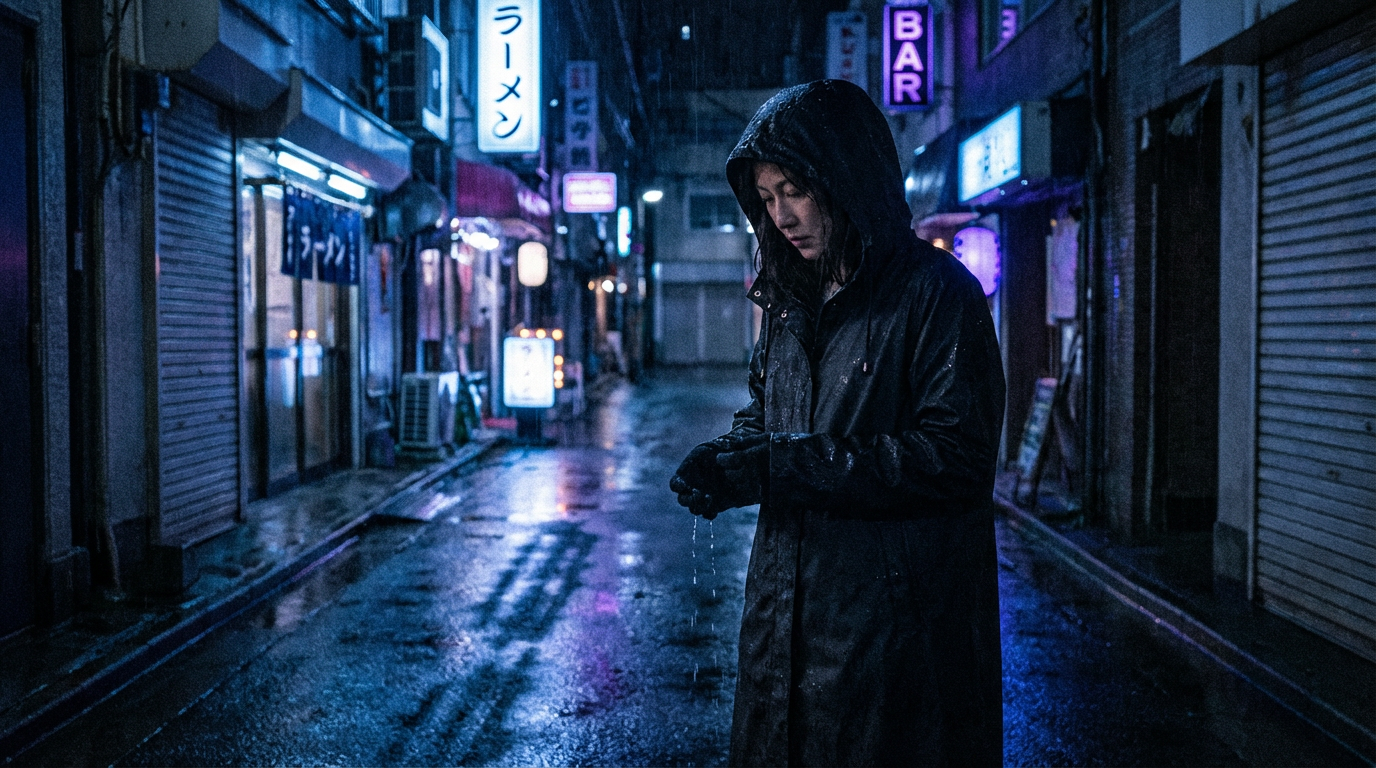
\includegraphics[width=\textwidth]{Fig3-10-2.png}
\subcaption{Second draft: Refined with tactile details}
\label{fig:ch03-neon-rain-v2}
\end{minipage}
\caption{Prompt iteration comparison: Adding sensory details and emotional depth transforms the output \\ \authorcreated}
\label{fig:ch03-neon-rain}
\end{figure}

The second version adds touch, color, and emotion; AI's response becomes more human. This is ``directorial writing''---controlling variables, adjusting rhythm, seeking authenticity.

\section{From Single Shot to Sequence: Making Text Tell Stories}
\index{narrative sequences}
\index{shot progression}

One Prompt describes one moment, while multiple Prompts can form \textbf{narrative beats}. Like film storyboards, you can link multiple sentences:

\begin{enumerate}
\item \textbf{Establishing shot} (Where)---Establish space and time
\item \textbf{Action shot} (What)---Show events or changes
\item \textbf{Emotional shot} (Why)---Reveal character state of mind
\item \textbf{Closing shot} (Closure)---Leave blank space or symbolism
\end{enumerate}

\begin{Prompt}
``Pre-dawn harbor, fog not yet dispersed. Fisherman lights lamp, light rippling on water surface. Camera rises, distant city begins to wake.''
\end{Prompt}

\begin{figure}[H]
\centering
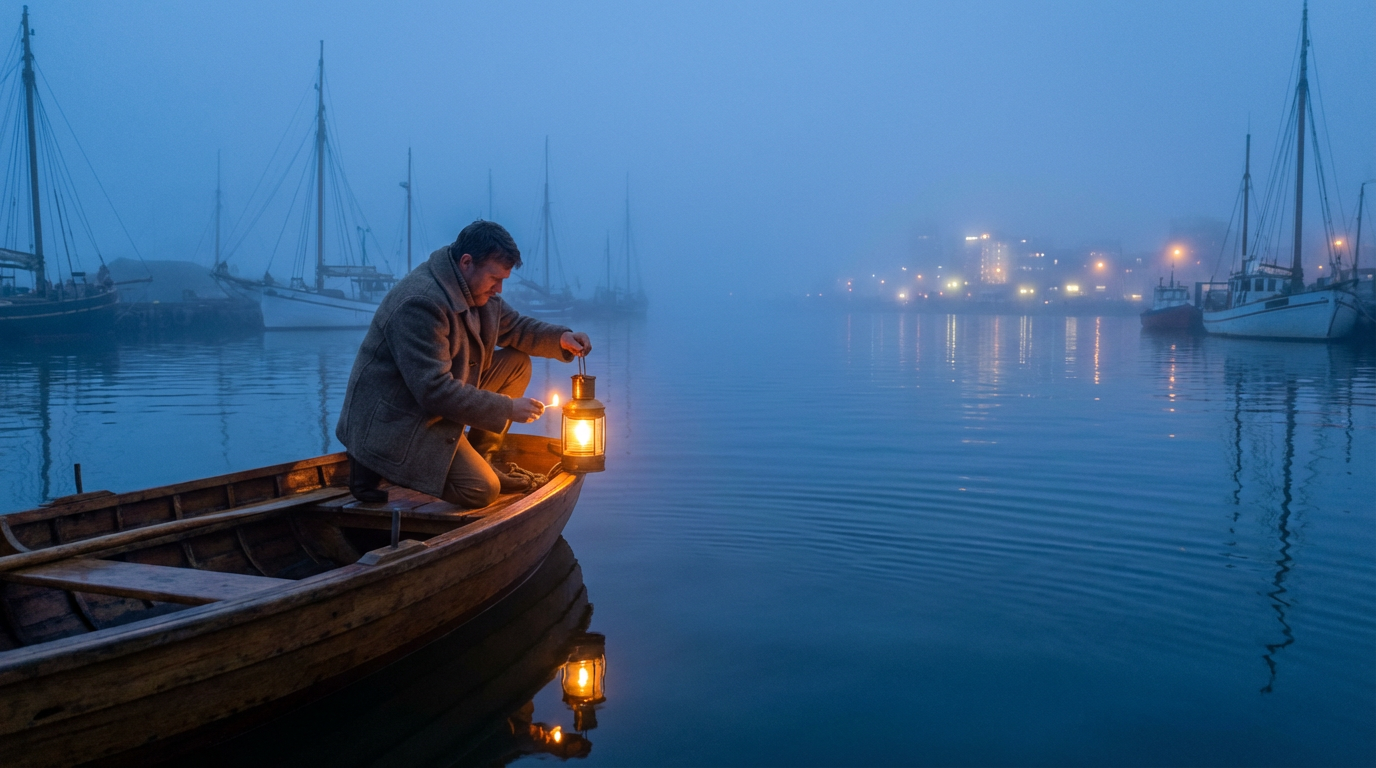
\includegraphics[height=\figheight]{Fig3-11.png}
\caption{Sequential narrative creating complete story arc \\ \authorcreated}
\label{fig:ch03-harbor}
\end{figure}

Four sentences, one story. Sora 2 will recognize rhythmic layers, balancing transitions between visual and emotional elements.

\section{Practice: Your First Sora 2 Prompt}
\index{practical exercise}

Now, open Sora 2 and input:

\begin{Prompt}
``A young woman stands on a rainy night street with flickering neon, water splashing at her feet, camera slowly circling around her.''
\end{Prompt}

\begin{figure}[H]
\centering
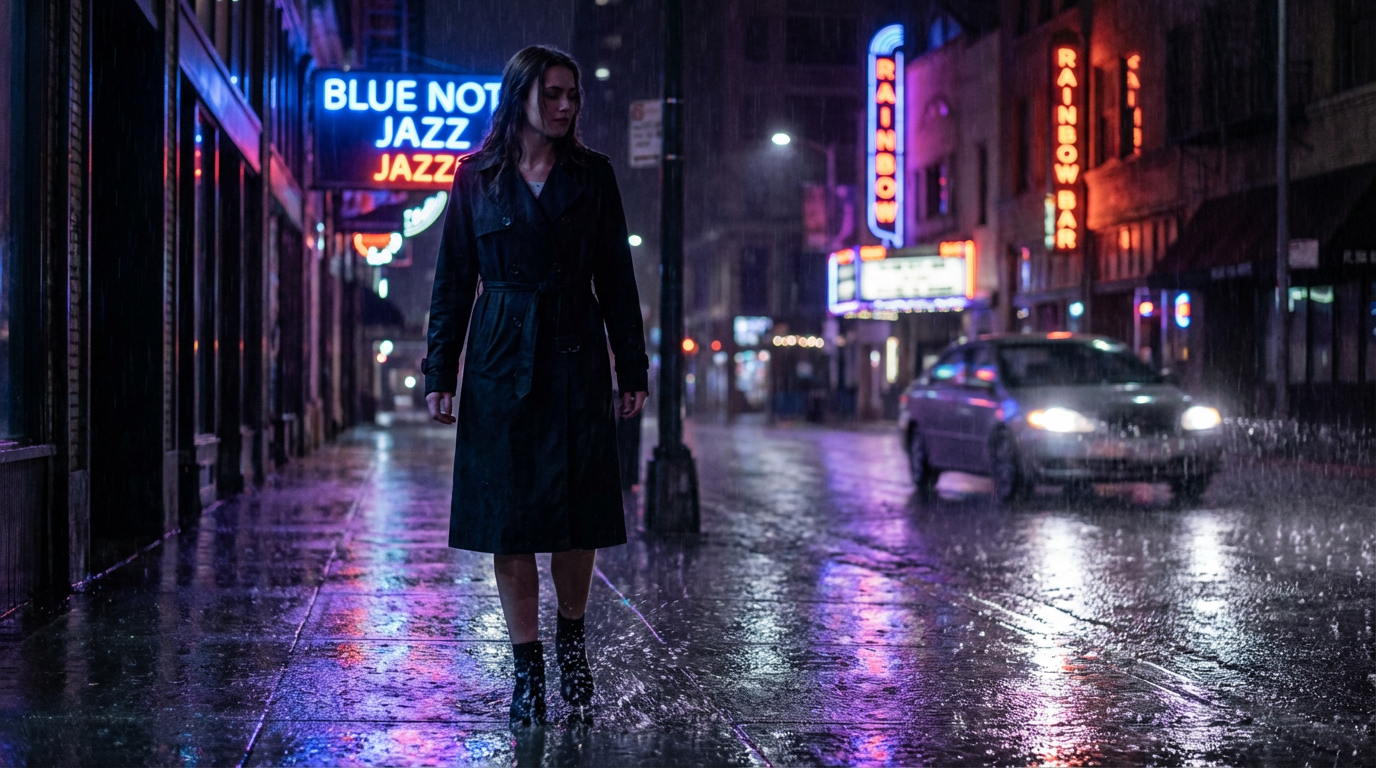
\includegraphics[height=\figheight]{Fig3-12.png}
\caption{Your first Sora 2 creation \\ \authorcreated}
\label{fig:ch03-first-Prompt}
\end{figure}

After generation, analyze carefully. Does it need more emotion? Is the rhythm too fast? Add words: ``cold blue tones,'' ``melancholic atmosphere,'' ``slow motion,'' ``low jazz music.'' Generate again.

You'll discover each word influences the frame's beat. Learning to shape through fine-tuning is true directorial skill.

\section{Summary: The Cinematic Nature of Text}
\index{textual cinema}

In Sora 2's world, \textbf{writing Prompts is like writing poetry}. Text doesn't just convey information; it constructs imagery.

\begin{itemize}
\item Write shots with rhythm
\item Write emotion with light
\item Write time with sentence structure
\end{itemize}

When you can write a scene with light, wind, and breath in thirty words, you've completed the leap from ``language'' to ``vision.'' Sora 2 becomes your camera, and your text becomes that invisible lens---capturing the world, capturing heartbeats.

\section*{Practical Exercises}
\index{practical exercises}

\begin{quote}
\textit{\textbf{Timeless Principle:} Even as interfaces evolve and platforms update, the underlying visual logic---light, composition, rhythm, and emotional resonance---remains eternal. Master these fundamentals, and you will adapt effortlessly to any future tool.}
\end{quote}

\subsection*{Exercise 1: Prompt Layer Building}
\textbf{Objective}: Master the five-layer Prompt construction method.

\textbf{Progressive Building Task}:
\begin{enumerate}
\item \textbf{Layer 1 - Subject}: "A young woman"
\item \textbf{Layer 2 - Action}: "A young woman reading a book"
\item \textbf{Layer 3 - Environment}: "A young woman reading a book in a cozy café"
\item \textbf{Layer 4 - Style}: "A young woman reading a book in a cozy café, warm golden lighting, shallow depth of field"
\item \textbf{Layer 5 - Emotion}: "A young woman reading a book in a cozy café, warm golden lighting, shallow depth of field, peaceful contemplation, soft smile"
\end{enumerate}

\textbf{Practice}: Create your own five-layer progression for: "An elderly man", "A child playing", "A couple walking"

\subsection*{Exercise 2: Cinematic Vocabulary Integration}
\textbf{Objective}: Learn to incorporate film terminology naturally into Prompts.

\textbf{Vocabulary Substitution}:
\begin{itemize}
\item Basic: "Person walking down street" 
\item Cinematic: "Tracking shot following figure down rain-soaked alley, handheld camera, film noir lighting"
\item Basic: "Cat on windowsill"
\item Cinematic: "Extreme close-up of tabby cat, shallow focus, golden hour backlighting, lens flare"
\end{itemize}

\textbf{Practice}: Transform these basic descriptions using cinematic vocabulary:
\begin{enumerate}
\item "Dog running in park"
\item "Woman cooking dinner"
\item "Child looking at stars"
\end{enumerate}

\subsection*{Exercise 3: Sensory Detail Enhancement}
\textbf{Objective}: Add texture, atmosphere, and sensory elements to Prompts.

\textbf{Sensory Expansion}:
\begin{Prompt}
Basic: "Forest scene"\\
Enhanced: "Misty forest morning, dappled sunlight filtering through ancient oak leaves, dewdrops catching light, soft rustling of branches, earthy moss textures"
\end{Prompt}

\textbf{Practice}: Add sensory details to these scenes:
\begin{itemize}
\item "Beach at sunset"
\item "City street at night"
\item "Mountain landscape"
\end{itemize}

\subsection*{Exercise 4: Genre Adaptation}
\textbf{Objective}: Learn to adapt the same scene across different cinematic genres

\textbf{Base Scene}: "A person walking down a hallway"

\textbf{Genre Variations to Create}:
\begin{itemize}
\item \textbf{Horror}: "Figure slowly walking down dimly lit hallway, shadows dancing on walls, creaking floorboards, handheld camera with slight shake, ominous atmosphere"
\item \textbf{Romance}: "Woman gracefully walking down sunlit hallway, soft focus, warm golden light streaming through windows, gentle camera glide, dreamy and hopeful mood"
\item \textbf{Thriller}: "Person hurriedly walking down narrow hallway, harsh fluorescent lighting, quick tracking shot, tension building, urgent footsteps echoing"
\item \textbf{Documentary}: "Subject walking naturally down office hallway, steady handheld camera, natural lighting, authentic movement, observational style"
\end{itemize}

\subsection*{Exercise 5: Prompt Diagnosis and Repair}
\textbf{Objective}: Identify and fix common Prompt problems

\textbf{Problematic Prompts to Fix}:
\begin{enumerate}
\item "Amazing beautiful sunset" → \textit{Add specificity and cinematic elements}
\item "Fast car driving really fast with lots of action" → \textit{Remove redundancy, add precise details}
\item "Person doing something interesting" → \textit{Define subject, action, and context}
\item "Epic scene with everything happening" → \textit{Focus and clarify the narrative}
\end{enumerate}

\section*{Prompt Construction Templates}
\index{Prompt templates}

\subsection*{Template 1: Narrative Scene Builder}
\begin{Prompt}
\textbf{[Character Description]} + [Emotional State] + [Action/Activity] + [Setting Details] + [Lighting/Atmosphere] + [Camera Technique] + [Symbolic Elements]

Example: "Weathered fisherman + contemplative + mending nets + weathered dock at dawn + soft pink light + slow dolly in + seagulls circling overhead"
\end{Prompt}

\subsection*{Template 2: Atmospheric Mood Creator}
\begin{Prompt}
\textbf{[Time/Season]} + [Weather/Environment] + [Color Palette] + [Texture Details] + [Movement/Rhythm] + [Emotional Undertone]

Example: "Autumn evening + light drizzle + warm amber and deep burgundy + wet cobblestones reflecting streetlights + gentle rhythm of footsteps + melancholic nostalgia"
\end{Prompt}

\subsection*{Template 3: Technical Precision Framework}
\begin{Prompt}
\textbf{[Shot Type]} + [Camera Movement] + [Focal Length Effect] + [Lighting Setup] + [Subject/Action] + [Background/Context]

Example: "Medium close-up + subtle push-in + 85mm compression + three-point lighting + pianist's hands on keys + concert hall ambiance"
\end{Prompt}

\section*{Quality Enhancement Checklist}
\index{quality checklist}

\subsection*{Pre-Generation Checklist}
Before submitting your Prompt, verify:

\begin{itemize}
\item[$\square$] \textbf{Specificity}: Does the Prompt contain concrete, visual details rather than vague adjectives?
\item[$\square$] \textbf{Cinematic Language}: Are camera angles, movements, and shot types clearly specified?
\item[$\square$] \textbf{Lighting Direction}: Is the lighting source, quality, and mood described?
\item[$\square$] \textbf{Emotional Clarity}: Is the intended mood or atmosphere explicitly stated?
\item[$\square$] \textbf{Action Definition}: Are movements and actions precisely described with appropriate pacing?
\item[$\square$] \textbf{Environmental Context}: Is the setting detailed enough to create a believable world?
\item[$\square$] \textbf{Length Balance}: Is the Prompt detailed enough without being overwhelming (50-150 words optimal)?
\end{itemize}

\subsection*{Post-Generation Evaluation}
After reviewing generated content:

\begin{itemize}
\item[$\square$] \textbf{Visual Coherence}: Do all elements work together harmoniously?
\item[$\square$] \textbf{Emotional Impact}: Does the video convey the intended mood?
\item[$\square$] \textbf{Technical Quality}: Are camera movements smooth and lighting consistent?
\item[$\square$] \textbf{Narrative Clarity}: Is the story or concept clearly communicated?
\item[$\square$] \textbf{Aesthetic Appeal}: Does the visual style match the intended genre or tone?
\end{itemize}

\subsection*{Iteration Strategy}
If results don't meet expectations:

\begin{enumerate}
\item \textbf{Identify the Gap}: What specific element differs from your vision?
\item \textbf{Targeted Adjustment}: Modify only the problematic aspect in your next Prompt
\item \textbf{A/B Testing}: Try two variations of the same Prompt to compare approaches
\item \textbf{Progressive Refinement}: Build complexity gradually rather than making dramatic changes
\item \textbf{Reference Integration}: Use successful elements from previous generations as building blocks
\end{enumerate}

\subsection*{Common Prompt Issues and Solutions}
\begin{table}[H]
\centering
\caption{Prompt Construction Problems and Fixes \\ \authorillustration}
\label{tab:Prompt-issues}
\begin{tabular}{p{4cm}p{4cm}p{5cm}}
\hline
\textbf{Issue} & \textbf{Example} & \textbf{Solution} \\
\hline
Too Generic & "Beautiful landscape" & "Rolling hills at golden hour, morning mist, wildflowers swaying, warm backlighting" \\
\hline
Overloaded & "Fast exciting action with lots of movement and energy" & "Runner sprinting, camera tracking alongside, determined expression, rhythmic breathing" \\
\hline
No Atmosphere & "Person sitting" & "Elderly man on park bench, dappled shade, gentle breeze, contemplative silence" \\
\hline
Missing Emotion & "Woman walking" & "Woman strolling confidently, slight smile, spring in her step, optimistic morning light" \\
\hline
\end{tabular}
\end{table}

\section*{Advanced Prompt Techniques}
\index{advanced techniques}

\subsection*{Technique 1: Temporal Progression}
Structure Prompts to show change over time:
\begin{Prompt}
"Seed in soil → first green shoot emerging → young plant reaching toward light → full bloom in garden"
\end{Prompt}

\subsection*{Technique 2: Perspective Shifting}
Use multiple viewpoints within one Prompt:
\begin{Prompt}
"Wide shot of busy café → close-up of barista's focused hands → customer's grateful smile → steam rising from fresh coffee"
\end{Prompt}

\subsection*{Technique 3: Symbolic Layering}
Embed metaphorical elements:
\begin{Prompt}
"Paper airplane floating through office cubicles, representing dreams escaping routine, soft lighting, slow motion"
\end{Prompt}



\section*{Chapter Summary}

Key actionable insights for Prompt construction:

\begin{itemize}
\item \textbf{Layered Structure}: Build Prompts with subject + action + environment + style + emotion for comprehensive control
\item \textbf{Cinematic Vocabulary}: Use film terminology (close-up, wide shot, golden hour, shallow depth) for precise visual direction
\item \textbf{Sensory Details}: Include texture, lighting, and atmospheric elements to create immersive scenes
\item \textbf{Iterative Refinement}: Start with basic Prompts and add specific details (color tones, mood, pacing) in subsequent generations
\item \textbf{Rhythm and Flow}: Structure sentences to match desired video pacing—short phrases for quick cuts, longer descriptions for sustained shots
\end{itemize}
